\documentclass[conference]{IEEEtran}
\IEEEoverridecommandlockouts
% The preceding line is only needed to identify funding in the first footnote. If that is unneeded, please comment it out.
\usepackage{cite}
\usepackage{hyperref}
\usepackage{amsmath,amssymb,amsfonts}
\usepackage{algorithmic}
\usepackage{graphicx}
\usepackage{xcolor}
\usepackage[]{footmisc}
\usepackage{multirow}
\usepackage{makecell}
\usepackage{booktabs}
\usepackage{hhline}
\usepackage{arydshln}
\usepackage{tablefootnote}
\usepackage[numbers]{natbib}

\setlength\heavyrulewidth{0.25ex}

\def\BibTeX{{\rm B\kern-.05em{\sc i\kern-.025em b}\kern-.08em
    T\kern-.1667em\lower.7ex\hbox{E}\kern-.125emX}}
    

\graphicspath{ {./img/} }
\begin{document}

\title{NLP for Fact-Checking and Claim Assessment\\
{\Large A Language Model based approach}
}

\author{
\IEEEauthorblockN{Othman El houfi}
\IEEEauthorblockA{\textit{MSc Data Science \& Machine Learning} \\
CY Cergy Paris University, France \\
othmanelhoufi@gmail.com}
\and
\IEEEauthorblockN{Dimitris Kotzinos}
\IEEEauthorblockA{\textit{University Professor} \\
CY Cergy Paris University, France \\
dimitrios.kotzinos@cyu.fr}
}

\maketitle

\begin{abstract}
As false information and fake news are propagating throughout the internet and social networks, the need of fact-checking operations becomes necessary in order to maintain a truthful digital environment where general information can be reliably exploited whether in politics, finance or other domains. The need of this online claim assessment comes from the fact that fake news and false information can have a big negative impact on politics, economy (2016 USA Elections) and public health (COVID-19).\\ 
A number of solutions have been proposed to deal with this problem and limit the spread of false information, both manual and automatic. Of course the manual approaches done on websites such as \textit{PolitiFact.com}, \textit{FactCheck.org} and \textit{Snopes.com} don't construct a viable solution for the long term as the speed and scale of information propagation increase exponentially rendering this manual fact-checking operation where human fact-checkers can't scale up at the same rate limited and incapable of solving the problem.\\
Here, we present our contribution in this regard: an automated solution for fact-checking using FEVER dataset as a source of truth and a state of the art language models used today for NLP tasks (BERT, RoBERTa, XLNet...) in order to classify a given claim as \textit{Supports}, \textit{Refutes} or \textit{Not enough information (NEI)}. We successfully prove that fine-tuning a LM with the correct settings can achieve an accuracy of 62\% and F-score of 61\% which is better than the majority of fact-checking methods that exists today.\\
\end{abstract}

\begin{IEEEkeywords}
Natural Language Processing, Language Model, Wikipedia, Information retrieval, Text processing, Natural Language Inferencing, Fact-Checking, Document retrieval, Fake-news.
\end{IEEEkeywords}

\section{Introduction}
From a social and psychological perspective, humans have been proven irrational and vulnerable when differentiating between truth and false news (typical accuracy ranges between 55\% and 58\%) \cite{zhou2019fake}, thus fake news obtain public trust relatively easier than truthful news because individuals tend to trust fake news after repeated exposure (\textit{Validity effect}), or if it confirms their pre-existing beliefs (\textit{Confirmation bias}), or simply due to the obligation of participating socially and proving a social identity (\textit{Peer pressure}). The social sciences are still trying to comprehend the biological motivations that makes fake news more appealing to humans.\\

On the other hand, the growth of social media platforms resulted in a huge acceleration of news spreading whether true or false. As of Aug. 2017, 67\% \cite{zhou2019fake} of Americans get their news from social media. These platforms even give the user the right to share, forward, vote and participate to online discussions. All of this made the problem of fake news spreading more and more dangerous, our economies for example, are not robust to the spread of falsity, false rumors have affected stock prices and the motivations for large-scale investments, as we witnessed after a false tweet claimed that Barack Obama was injured in an explosion which caused \$130 billion drop in stock value \cite{vosoughi2018spread}. Another recent example is related to public health where rumors about COVID-19 vaccines and drug companies influenced people in their decision on getting vaccinated.\\

That being said, is there a way to monitor the spread of fake news through social media? Or more specifically, how can we differentiate between fake news and truthful news, and at what level of confidence can we do that?\\

From a computer engineering perspective, different approaches were studied:

\begin{itemize}
\item \textbf{Knowledge-based Fake News Detection \cite{chernyavskiy2021whatthewikifact}:} a method aims to assess news authenticity by comparing the knowledge extracted from to-be verified news content with known facts, also called fact-checking.
\item \textbf{Style-based Fake News Detection \cite{przybyla2020capturing}:} focuses on the style of writing, i.e. the form of text rather than its meaning.
\item \textbf{Propagation-based Fake News Detection \cite{shu2020hierarchical}:} a principled way to characterize and understand hierarchical propagation network features. We perform a statistical comparative analysis over these features, including micro-level and macro-level, of fake news and true news.
\item \textbf{Credibility-based Fake News Detection \cite{sitaula2020credibility}:} the information about authors of news articles can indicate news credibility and help detect fake news.
\end{itemize}

In this paper we will focus on a new approach that utilizes Language Models (LMs) for fact-checking. The goal is not to implement an algorithm that scans social networks for real time fake news detection, but rather we will create a model that can assess with a degree of confidence the truthfulness or falseness of a claim given by a user as an input by exploiting LMs that were already trained on Wikipedia, and fine-tune each LM for a downstream task in order to solve this classification problem.

\section{Related works}
\subsection{Language model based approach \cite{lee2020language} \cite{petroni2019language}}
A paper entitled \textit{"Language Models as Fact Checkers?"} published by a team from \textit{FacebookAI} and \textit{Hong Kong University of Science and Technology}, provides an example of a fact-checking model using zero-shot LM that outperforms a random baseline LM using the FEVER dataset\cite{thorne2018fever}.\\

The goal of fact-checking as mentioned previously, and relatively to this paper, is to validate the truthfulness of a given claim. Each claim is assigned to one of these labels: \textit{Supports}, \textit{Refutes} or \textit{Not enough information (NEI)} to verify.\\

This paper describes the difference between Traditional Pipeline fact-checking models and their zero-shot fact-checking LM:

\begin{itemize}
\item \textbf{Traditional pipeline:} this type of models access knowledge within an external knowledge base like Wikipedia in order to validate a claim. It involves information retrieval modules such as document retrieval and sentence retrieval.
\item \textbf{Zero-shot LM pipeline:} it replaces both the external knowledge base and the information retrieval modules with a pre-trained language model.\\
\end{itemize}

They used the publicly available 24-layer BERT-Large as LM, which was pre-trained on Wikipedia in 2018. After fine-tuning the model they achieved 57\% in accuracy and 57\% in F1-macro score which was better than the baseline BERT model (without fine-tuning) that achieved 49\% in accuracy and 44\% in F1-macro score.

\subsection{Perplexity based approach \cite{lee2021towards} \cite{lee2020misinformation}}
In March 2021, \textit{Nayeon Lee}, \textit{Yejin Bang}, \textit{Andrea Madotto}, \textit{Madian Khabsa}, and \textit{Pascale Fung} published a paper called \textit{Towards Few-Shot Fact-Checking via Perplexity} where they propose a new approach of the powerful transfer learning ability of a language model via a perplexity score. Using a method called \textit{few-shot learning}, they built a model that outperforms major class baseline models by more than 10\% on the F1-Macro metric score.\\
In this paper the goal is to determine the veracity of a claim given some evidence, for this they define a {claim, evidence} pair. The label \emph{Supported} is assigned when relevant evidence exists that supports the claim, and \emph{Unsupported} label for the opposite case.\\
\emph{Unsupported} claims on average have higher perplexity than \emph{Supported} claims. For example, \emph{Supported} claim "Washing hands prevents the spread of diseases" has a perplexity value of 96.74, whereas the \emph{Unsupported} claim "All dogs speak English fluently" has a much higher perplexity value of 328.23.\\
The datasets used in this experiment are: Covid19-Scientific, Covid19-Social, and FEVER. As for the perplexity based experiment they used one unidirectional LM and one masked LM:
\begin{itemize}
\item $PPL_{GPT2-B}$ : a single-parameter classifier based on perplexity from GPT2-base \cite{radford2019language} (unidirectional LM)
\item $PPL_{BERT-B}$ : a single-parameter classifier based on perplexity from BERT-base \cite{devlin2018bert} (Masked LM)\\
\end{itemize}

They took into consideration the accuracy and the F1-Macro metrics for the evaluation. Because the datasets are unbalanced, they mainly consider the F1-Macro score over accuracy as an overall evaluation. The perplexity-based classifiers, especially $PPL_{GPT2-B}$, outperform all Major Class baselines across all
tasks in all settings. For instance, $PPL_{GPT2-B}$ achieved accuracy of 67.48\% and F1-macro score of 64.70\% on FEVER dataset.\\
On the other hand the classification was limited to two labels (\emph{Supported} and \emph{Unsupported}) which does not solve the entire classification problem in the FEVER dataset that provides three labels (\textit{Supports}, \textit{Refutes} or \textit{Not enough information (NEI)}).

\section{Proposed method}
Most of the fact-checking algorithms today involving knowledge-based verification uses a traditional pipeline that puts in place a module for retrieving articles from an external source, another module for retrieving relevant sentences from each article, and a last module for natural language inferencing (NLI) in order to classify a claim.

\begin{figure}[htp]
    \centering
    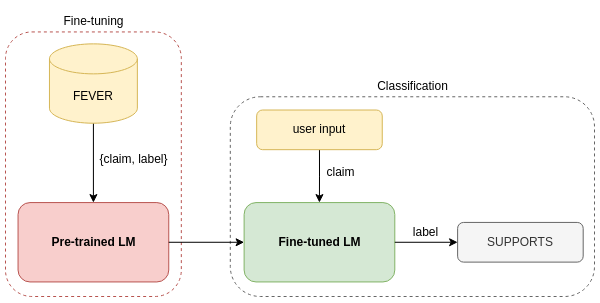
\includegraphics[scale=0.4]{processing_pipeline.png}
    \caption{Proposed method pipeline.}
    \label{fig:processing_pipeline}
\end{figure}


In this paper we present a method that is fully  reliant on the powerfulness of today's best LMs. As illustrated in Figure \ref{fig:processing_pipeline}, we start by fine-tuning each model for the downstream task that is claim classification using the FEVER dataset, then each model is employed to assess the validity of new input claims. This approach takes into consideration only an internal knowledge source (FEVER) for fine-tuning, that is for the learning phase, which makes the prediction phase knowledge-free rather than utilizing external knowledge sources for retrieving articles and sentences.

It is also important to mention that we only use LMs for classifying claims and not for generating evidence. We leave generating evidences with language models for future work.

\subsection{FEVER Dataset}
FEVER (Fact Extraction and VERification) consists of 185,445 claims generated by altering sentences extracted from Wikipedia and subsequently verified without knowledge of the sentence they were derived from. The claims are classified as Supported, Refuted or NotEnoughInfo. For the first two classes, the annotators also recorded the sentence(s) forming the necessary evidence for their judgment\cite{thorne2018fever}.

\begin{figure}[htp]
    \centering
    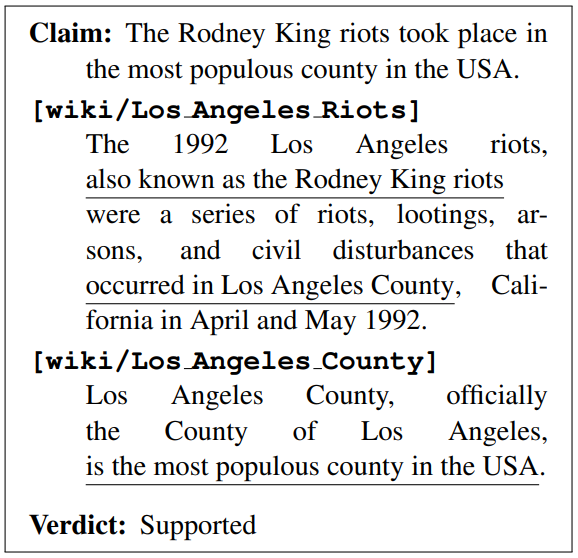
\includegraphics[scale=0.3]{fever_example.png}
    \caption{Manually verified claim requiring evidence from multiple Wikipedia pages.}
    \label{fig:fever_example}
\end{figure}

Since our mission is to classify claims to \textit{SUPPORTS}, \textit{REFUTES} or \textit{NEI} and not generating evidence, we omit the evidences information in the dataset. Then we map each label to an integer: \{\textit{SUPPORTS} : 1, \textit{REFUTES} : 0, \textit{NEI} : 2\} and that is all we do as far as data pre-preprocessing goes.

\begin{table}[htp]
\centering
\resizebox{0.48\textwidth}{!}{%
\begin{tabular}{|c||c|c|}
\hline
\textbf{ID} & \textbf{Claim} & \textbf{Label} \\ \hline \hline
79044      & The Apple Store first opened in 2001.  & 1 \\ \hline
117129         & Adventure Time won an Oscar.    & 0  \\ \hline
55061           & Yamaha Corporation produces hardware.    & 2 \\ \hline
\end{tabular}
}
\vspace{0.4cm}
\caption{Examples of FEVER claims and labels.}
\label{tab:fever_example}
\end{table}

Finally we split the dataset to training, validation and testing sets that we can use for LM fine-tuning and testing:

\begin{table}[htp]
\centering
\resizebox{0.48\textwidth}{!}{%
\begin{tabular}{|c||c|c|c|c|}
\hline
\textbf{Split} & SUPPORTS & REFUTES & NEI    & \textbf{Total} \\ \hline \hline
Train          & 80,035   & 29,775  & 35,639 & 145,449        \\ \hline
Val            & 3,333    & 3,333   & 3,333  & 9,999          \\ \hline
Test           & 3,333    & 3,333   & 3,333  & 9,999          \\ \hline
\end{tabular}%
}
\vspace{0.4cm}
\caption{Dataset split sizes for SUPPORTS, REFUTES and NOTENOUGHINFO (NEI) classes.}
\label{tab:fever_splits}
\end{table}

\subsection{Language Models}
The year 2018 has been an inflection point for NLP as Google introduced a LM called BERT (Bidirectional Encoder Representations from Transformers)\cite{devlin2018bert}. This model was described as state-of-the-art model that solves the most difficult tasks in NLP, it is also used today in Google's search engine for text completion and translation. BERT model can be fine-tuned with just one additional output layer to create state-of-the-art models for a wide range of tasks, such as question answering and language inference, without substantial task specific architecture modifications. From there a lot of LMs were introduced that uses the same architecture as BERT but with small changes such as number of parameters and data on which the model was pre-trained.

\begin{figure}[htp]
    \centering
    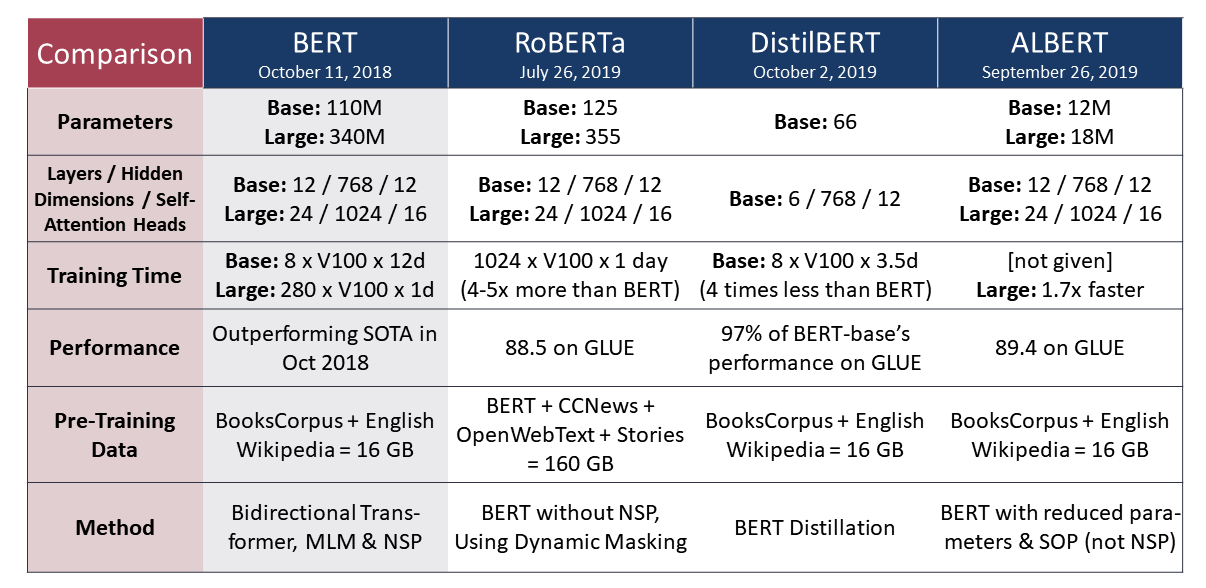
\includegraphics[scale=0.28]{lm_compar.png}
    \caption[Comparison]{Comparison of BERT, RoBERTa, DistilBERT, and ALBERT. \footnotemark}
    \label{fig:lm_compar}
\end{figure}
\footnotetext{\url{https://humboldt-wi.github.io/blog/research/information_systems_1920/uncertainty_identification_transformers/}}

In this paper we will classify claims by fine-tuning the following LMs:

\begin{itemize}
\item BERT-base-uncased \cite{devlin2018bert}
\item RoBERTa-base \cite{liu2019roberta}
\item DistilBERT-base-uncased \cite{sanh2019distilbert}
\item XLNET-base-cased \cite{yang2019xlnet}
\item ALBERT-base-v2 \cite{lan2019albert}
\item BigBird-RoBERTa-base \cite{zaheer2020big}\\
\end{itemize}

All of these LMs were trained on Wikipedia dataset containing cleaned articles. The datasets are built from the Wikipedia dump \footnote{\url{https://dumps.wikimedia.org/}} with one split per language. Each example contains the content of one full Wikipedia article with cleaning to strip markdown and unwanted sections (references, etc.). So in one way, all these LMs were trained on facts from Wikipedia, for example if we give the following input \textit{"Paris is the capital of [MASK]."} to BERT-base model, the output will be \textit{"Paris is the capital of France."} with a probability of 0.951.\\
So the conjecture behind our method is that: fine-tuning LMs that were pre-trained on Wikipedia, and by exploiting the already stored knowledge within these LMs, we can create a self-knowledge-independent fact-checking classifier.
\section{Experiment Protocol and Results}
\subsection{Experiment Setup}
As mentioned before, we conduct our experiment on the FEVER dataset using the splits in Table \ref{tab:fever_splits}. As for LMs fine-tuning we used one GPU, the NVIDIA RTX6000P-8C with 24Go of GDDR6 memory and a peak single precision floating point performance of 14,9 Tflops.\\

For all models we chose the following hyperparameters:

\begin{itemize}
\item Tokenizer max sequence length: 128
\item Output layer size: 3 (classes: 0, 1 and 2)
\item Activation function: GeLU
\item Learning rate: 3e-5
\item Optimization: Adam with linear decay
\item Loss function: Cross-Entropy
\item Epochs: 3
\item Training batch size: 20
\item Validation batch size: 20\\
\end{itemize}

These hyperparameters may not be optimal, but they were chosen after many different repeated experiments. Optimizing the models is left for future work.
\subsection{Evaluation Metric}
Most of the fact-checking methods that uses FEVER dataset employ FEVER scoring\cite{thorne2018fever}, a metric that considers classification accuracy and evidence recall, but since we don't tackle the evidence problem in our approach, we rely on accuracy, recall, precision and F1-score of the model classification as metrics for evaluation.\\
In addition, we track other aspects of each LM such as training time, model size, and memory usage during the fine-tuning step in order to make an overall evaluation.
\subsection{Results and Discussion}
\begin{table*}[htp]
	\centering
	\resizebox{0.9\textwidth}{!}{%
	\begin{tabular}{c!{\vrule width \heavyrulewidth}cccccccc} 
	\bottomrule
	\textbf{Fine-tuned model} & \textbf{Label} & \textbf{prec} & \textbf{recall} & \textbf{~f1} & \textbf{accuracy} & \textbf{macro prec} & \textbf{macro recall} & \textbf{macro f1} \\ 
	\toprule
	\multirow{3}{*}{\textit{BERT-base-uncased}} & SUPPORTS & 0.55 & 0.78 & 0.64 & \multirow{3}{*}{\textbf{0.62}} & \multirow{3}{*}{0.63} & \multirow{3}{*}{\textbf{0.62}} & \multirow{3}{*}{\textbf{0.61}} \\
	 & REFUTES & 0.75 & 0.59 & 0.66 &  &  &  &  \\
	 & NEI & 0.61 & 0.47 & 0.53 &  &  &  &  \\ 
	\midrule
	\multirow{3}{*}{\textit{ALBERT-base-v2}} & SUPPORTS & 0.46 & 0.81 & 0.59 & \multirow{3}{*}{0.53} & \multirow{3}{*}{0.58} & \multirow{3}{*}{0.53} & \multirow{3}{*}{0.52} \\
	 & REFUTES & 0.77 & 0.46 & 0.58 &  &  &  &  \\
	 & NEI & 0.50 & 0.33 & 0.40 &  &  &  &  \\ 
	\midrule
	\multirow{3}{*}{\textit{DistilBERT-base-uncased}} & SUPPORTS & 0.54 & 0.78 & 0.64 & \multirow{3}{*}{0.61} & \multirow{3}{*}{0.63} & \multirow{3}{*}{0.61} & \multirow{3}{*}{\textbf{0.61}} \\
	 & REFUTES & 0.75 & 0.58 & 0.65 &  &  &  &  \\
	 & NEI & 0.60 & 0.47 & 0.53 &  &  &  &  \\ 
	\midrule
	\multirow{3}{*}{\textit{RoBERTa-base}} & SUPPORTS & 0.54 & 0.81 & 0.65 & \multirow{3}{*}{\textbf{0.62}} & \multirow{3}{*}{\textbf{0.64}} & \multirow{3}{*}{\textbf{0.62}} & \multirow{3}{*}{\textbf{0.61}} \\
	 & REFUTES & 0.75 & 0.59 & 0.66 &  &  &  &  \\
	 & NEI & 0.63 & 0.45 & 0.53 &  &  &  &  \\ 
	\midrule
	\multirow{3}{*}{\textit{BigBird-RoBERTa-base}} & SUPPORTS & 0.53 & 0.81 & 0.64 & \multirow{3}{*}{0.61} & \multirow{3}{*}{\textbf{0.64}} & \multirow{3}{*}{0.61} & \multirow{3}{*}{0.60} \\
	 & REFUTES & 0.75 & 0.58 & 0.66 &  &  &  &  \\
	 & NEI & 0.63 & 0.44 & 0.52 &  &  &  &  \\ 
	\midrule
	\multirow{3}{*}{\textit{XLNET-base-cased}} & SUPPORTS & 0.53 & 0.81 & 0.64 & \multirow{3}{*}{0.61} & \multirow{3}{*}{0.63} & \multirow{3}{*}{0.61} & \multirow{3}{*}{0.60} \\
	 & REFUTES & 0.74 & 0.59 & 0.65 &  &  &  &  \\
	 & NEI & 0.63 & 0.43 & 0.51 &  &  &  &  \\
	\bottomrule
	\textbf{Related work} & \textbf{Label} & \textbf{prec} & \textbf{recall} & \textbf{~f1} & \textbf{accuracy} & \textbf{macro prec} & \textbf{macro recall} & \textbf{macro f1} \\ 
	\toprule
	\multirow{3}{*}{\textit{BERT-large} \cite{lee2020language}} & SUPPORTS & 0.54 & 0.67 & 0.59 & \multirow{3}{*}{0.57} & \multirow{3}{*}{0.57} & \multirow{3}{*}{0.57} & \multirow{3}{*}{0.57} \\
	 & REFUTES & 0.62 & 0.55 & 0.58 &  &  &  &  \\
	 & NEI & 0.57 & 0.49 & 0.53 &  &  &  &  \\ 
	\midrule
	\textit{FEVER Baseline} \cite{thorne2018fact} & - & - & - & - & 0.49 & - & - & -\\
	\textit{Ohio State University} \cite{thorne2018fact} & - & - & - & - & 0.50 & - & - & -\\
	\textit{Columbia NLP} \cite{thorne2018fact} & - & - & - & - & 0.58 & - & - & -\\
	\textit{Papelo} \cite{thorne2018fact} & - & - & - & - & 0.61 & - & - & -\\
	\textit{UNC-NLP} \cite{thorne2018fact} & - & - & - & - & 0.68 & - & - & -\\
	\textit{DREAM} \cite{zhong2019reasoning} & - & - & - & - & \textbf{0.77} & - & - & -\\
	
	\end{tabular}%
	}
	\vspace{0.4cm}
	\caption{Classification metrics for each fine-tuned LM using our approach vs. BERT-large fine-tuned by FacebookAI team vs. other models based on knowledge graphs and/or traditional pipelines that uses FEVER dataset (we take into consideration only the accuracy of label classification and not the FEVER scoring system).}
	\label{tab:accuracy_res}
\end{table*}


The results of the six models are reported in Table \ref{tab:accuracy_res}. We can observe that our approach yields to better results than FacebookAI's model and most of the traditional methods that involves external information retrieval modules.\\

Specifically the fine-tuned \textit{RoBERTa-base} model surpasses the fine-tuned \textit{BERT-large} model created by FacebookAI in every metric. For instance our model achieved an accuracy score of 62\% and a macro precision score of 64\% which is an improvement of 5\% and 7\% respectively. Not only that, it is also worth mentioning that \textit{RoBERTa-base} has only 125 million parameters and 12 encoding layers in comparison to \textit{BERT-large} that has 340 million parameters and 24 encoding layers, thus rendering our model more efficient to train, to store and to implement.\\

The improvements in classification is probably due to the fact that \textit{RoBERTa} is pre-trained on more data than \textit{BERT} as shown in Figure \ref{fig:lm_compar}. On the other hand, our fine-tuned \textit{BERT-base} model also achieved better results than FacebookAI's model which may be explained by the difference of hyperparameters choice.\\

Similarly, the fine-tuned \textit{RoBERTa-base} model achieved more accuracy score for label classification than most of the traditional pipelines, therefore it puts our approach on the top-10 best fact-checking models that were published by FEVER community\cite{thorne2018fact} (without taking into consideration the evidence generation metric). It is also safe to say that the \textit{DREAM} fact-checking model is certainly superior than all our LMs as it achieved an accuracy score of 77\% which is 15\% higher. This is a proof that there is still much room for future research and improvements.\\

Same as FacebookAI results\cite{lee2020language}, and upon examining the results of our fine-tuned LMs closely, we also find that all our LMs struggles immensely with the NEI category (lowest F1 scores) indicating that our current approach might also need specific modules to better tackle that category.\\

% This was also confirmed when we plotted the confusion matrix of our models (for example \textit{RoBERTa-base} in Figure \ref{fig:confusion_matrix_roberta}).
%\begin{figure}[htp]
%    \centering
%    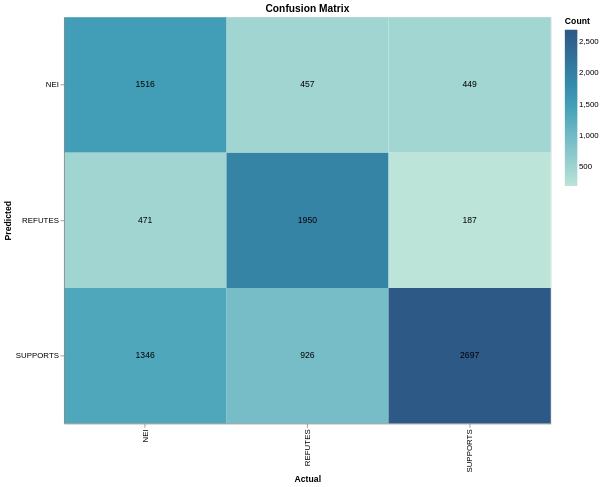
\includegraphics[scale=0.3]{confusion_matrix_roberta.png}
%    \caption[Comparison]{Confusion Matrix of the fine-tuned \textit{RoBERTa-base} using test set.}
%    \label{fig:confusion_matrix_roberta}
%\end{figure}

Furthermore, the difference in classification performance between our LMs is not big considering the fact that each LM was pre-trained differently. The only model that performed poorly is \textit{ALBERT-base-v2}, it achieved only 53\% accuracy score and 52\% macro F1 score. This can be explained by the reduced number of the model's parameters (12 million vs. \textit{BERT}'s 110 million).\\

We can also see the differences between each LM during the training and the evaluation as illustrated in Figure \ref{fig:train_loss} and Figure \ref{fig:eval_loss}.

\begin{figure}[htp]
    \centering
    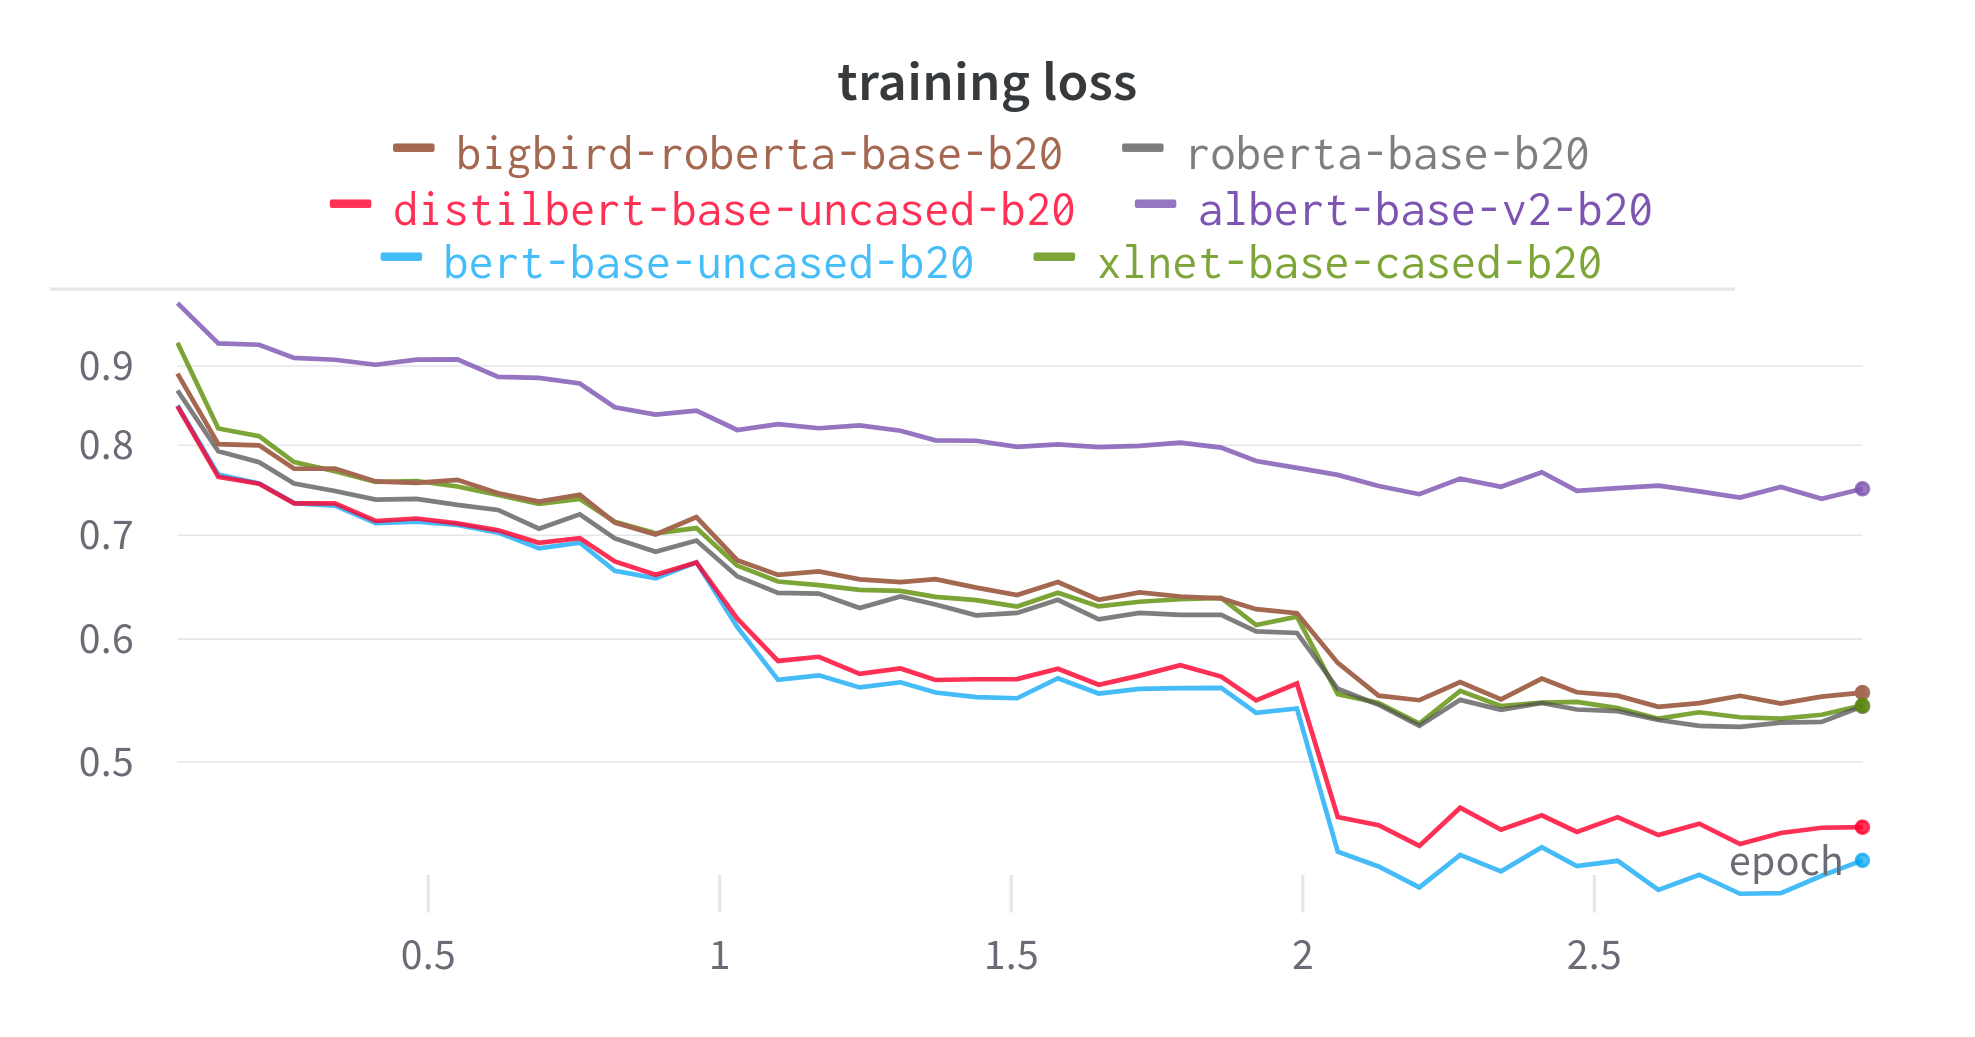
\includegraphics[scale=0.13]{train_loss.png}
    \caption[Comparison]{The Cross-Entropy Loss of each LM during training.}
    \label{fig:train_loss}
\end{figure}

\begin{figure}[htp]
    \centering
    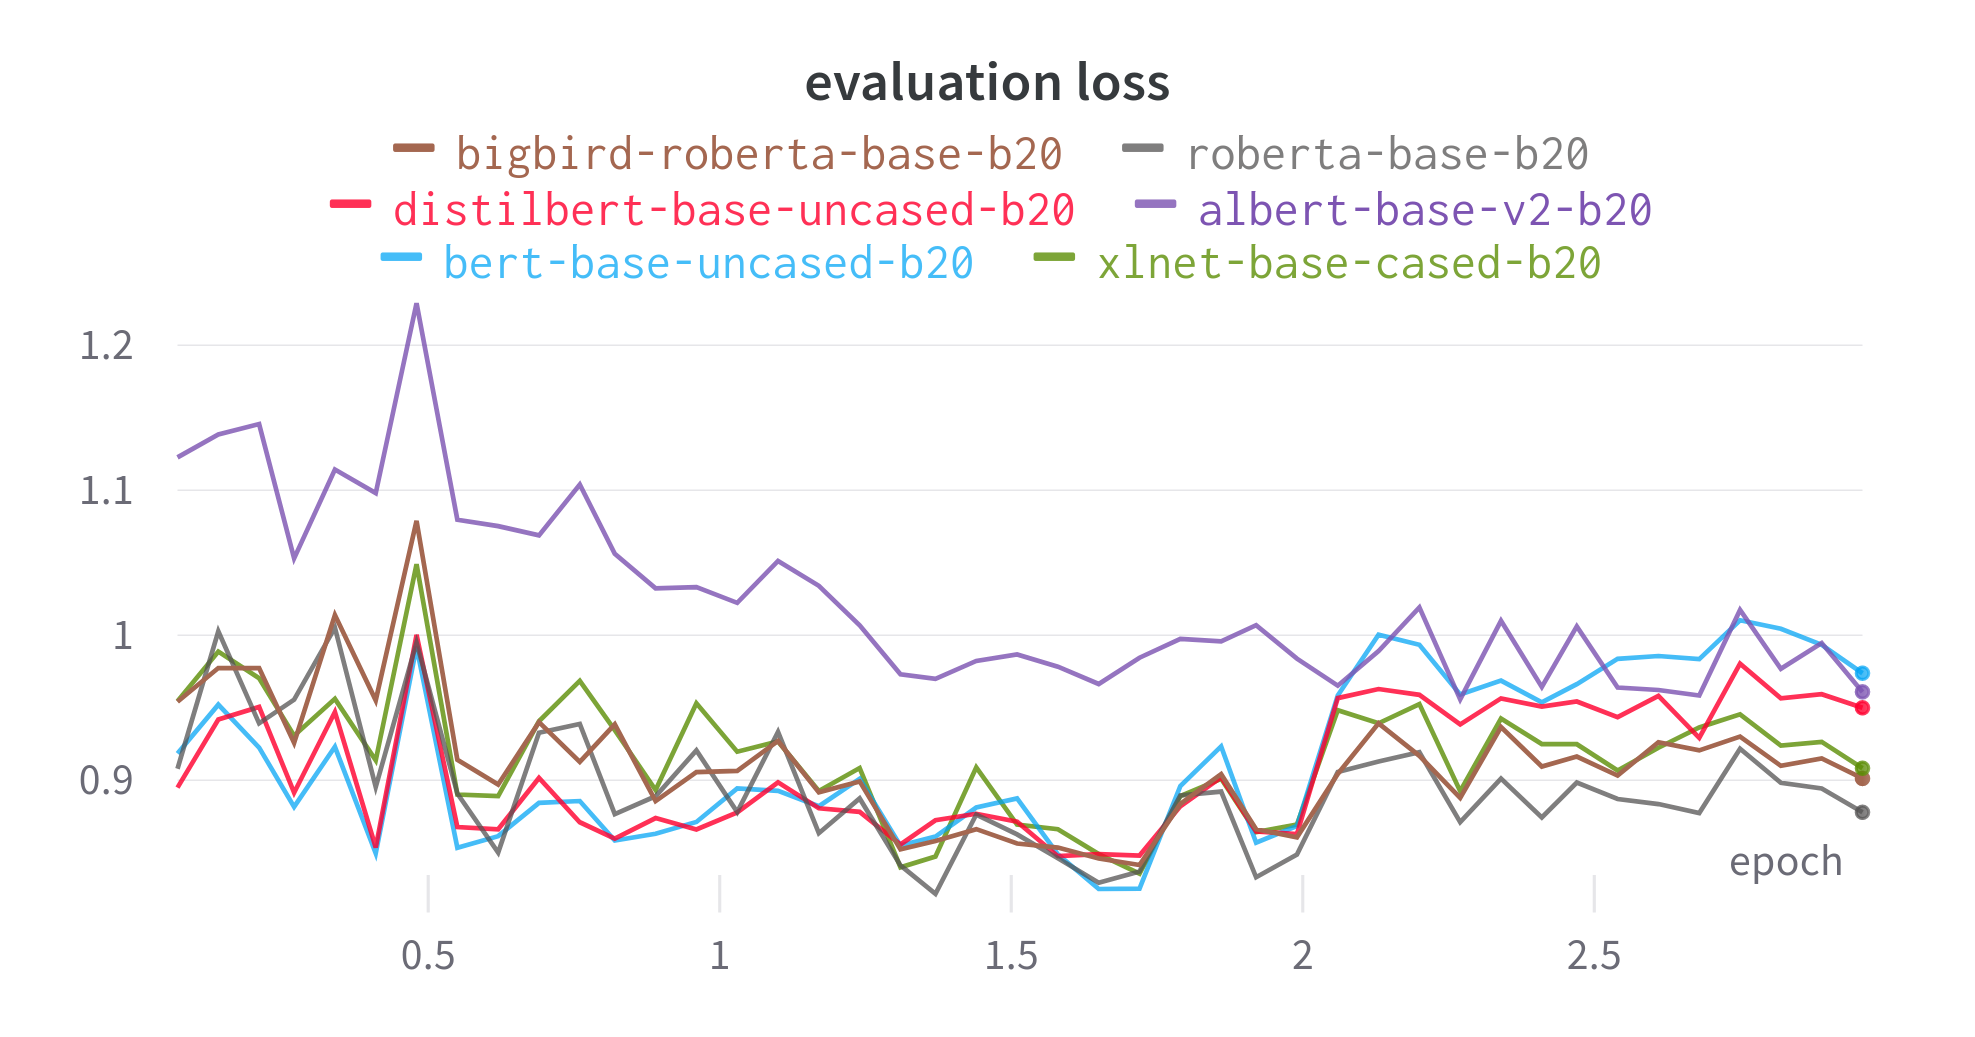
\includegraphics[scale=0.13]{eval_loss.png}
    \caption[Comparison]{The Cross-Entropy Loss of each LM during evaluation.}
    \label{fig:eval_loss}
\end{figure}

As expected, \textit{RoBERTa-base} model reached the lowest Cross-Entropy loss of 0.878 during evaluation while \textit{ALBERT-base-v2} kept a higher loss of 0.961 during evaluation (also 0.75 during training). It is even clearer in Figure \ref{fig:eval_mcc} and Figure \ref{fig:eval_acc}  that \textit{ALBERT-base-v2} had the lowest Matthews correlation coefficient score (mcc) as well as  accuracy score during evaluation.

\begin{figure}[htp]
    \centering
    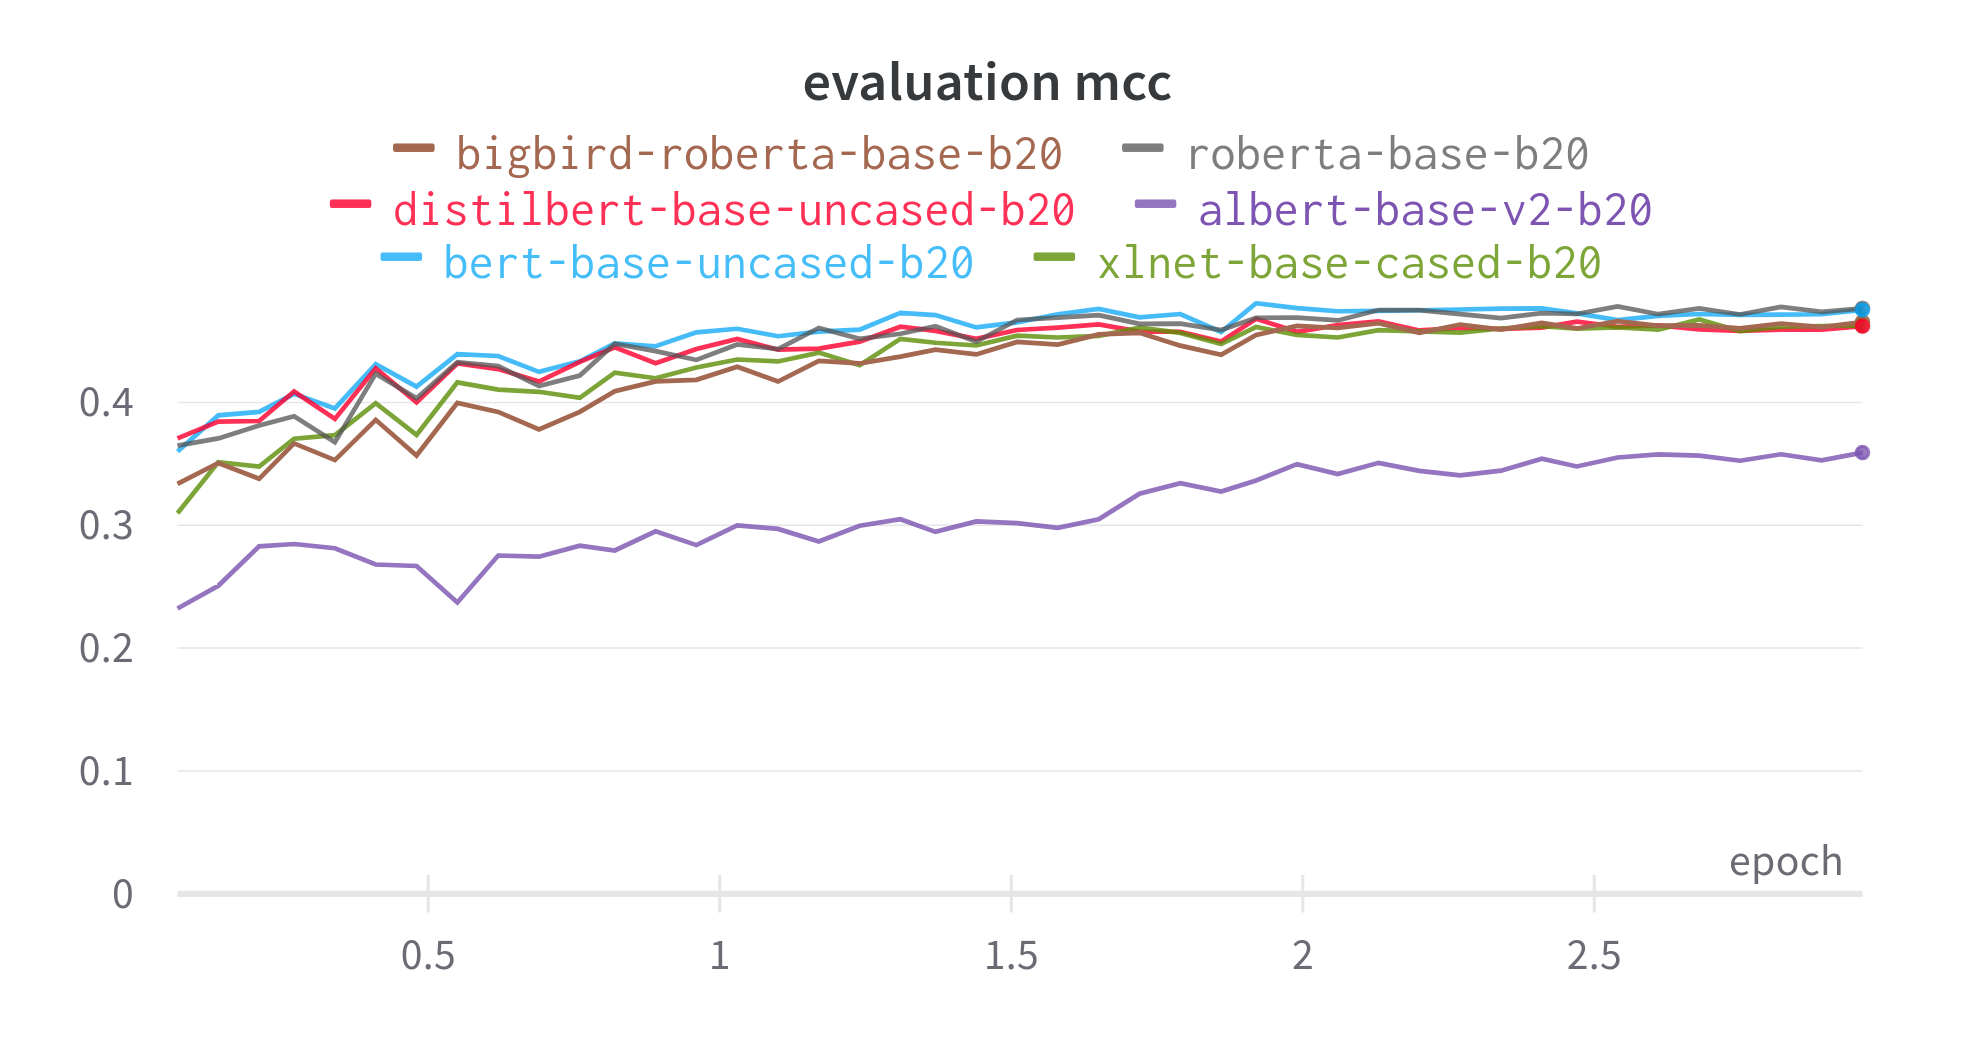
\includegraphics[scale=0.13]{eval_mcc.png}
    \caption[Comparison]{The Matthews correlation coefficient score of each LM during evaluation.}
    \label{fig:eval_mcc}
\end{figure}

\begin{figure}[htp]
    \centering
    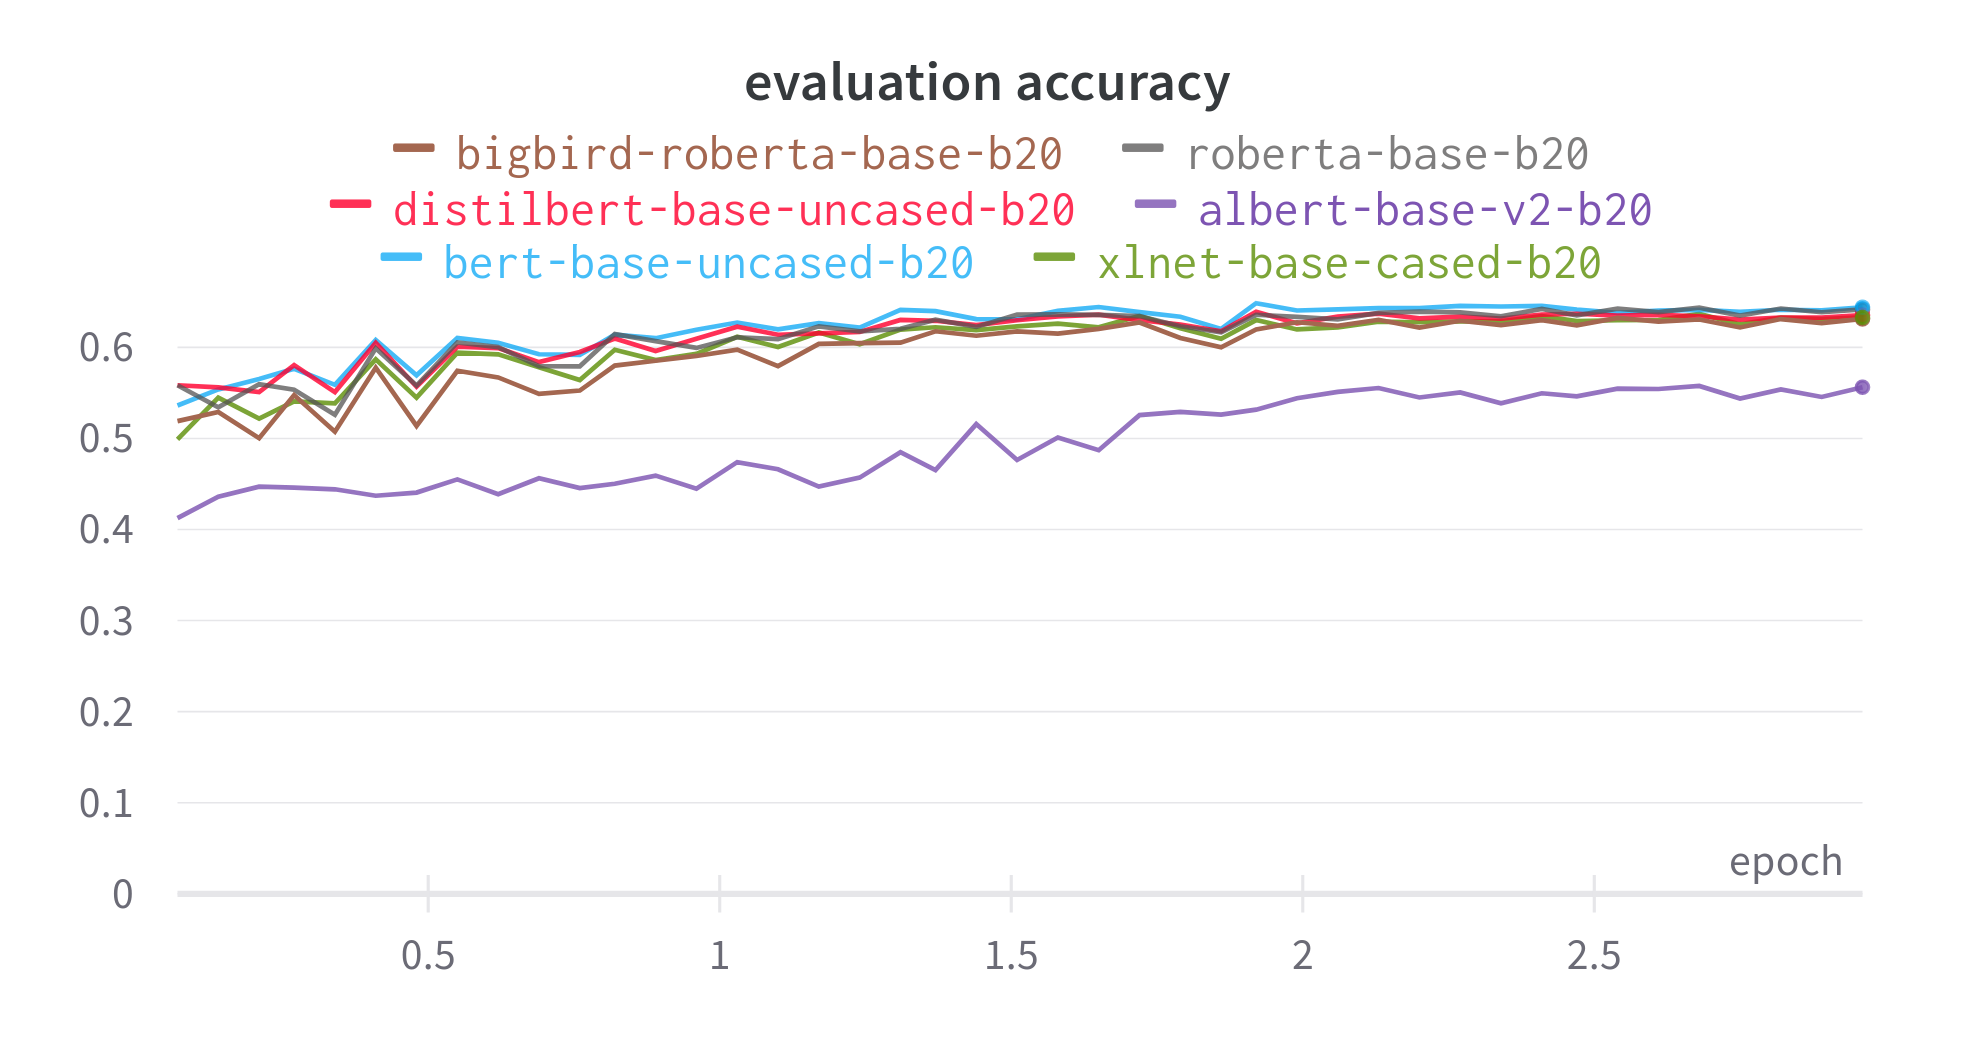
\includegraphics[scale=0.13]{eval_acc.png}
    \caption[Comparison]{The accuracy score of each LM during evaluation.}
    \label{fig:eval_acc}
\end{figure}

Even if the other LM reached the same accuracy and mcc as \textit{RoBERTa-base} during evaluation or a lower loss during training they did not perform as well in the test set which was demonstrated in Table \ref{tab:accuracy_res}.\\

Finally, it is also important to mention that training time differs from one LM to another (Figure \ref{fig:train_time}) as the number of parameters are not similar, for instance \textit{XLNET-base-cased} model spent 1h56m for training while \textit{RoBERTa-base} took 1h25m and achieved better results. The idea that we are trying to prove is that we don't need a bigger model in order to achieve greater results for a downstream task like text classification.

\begin{figure}[htp]
    \centering
    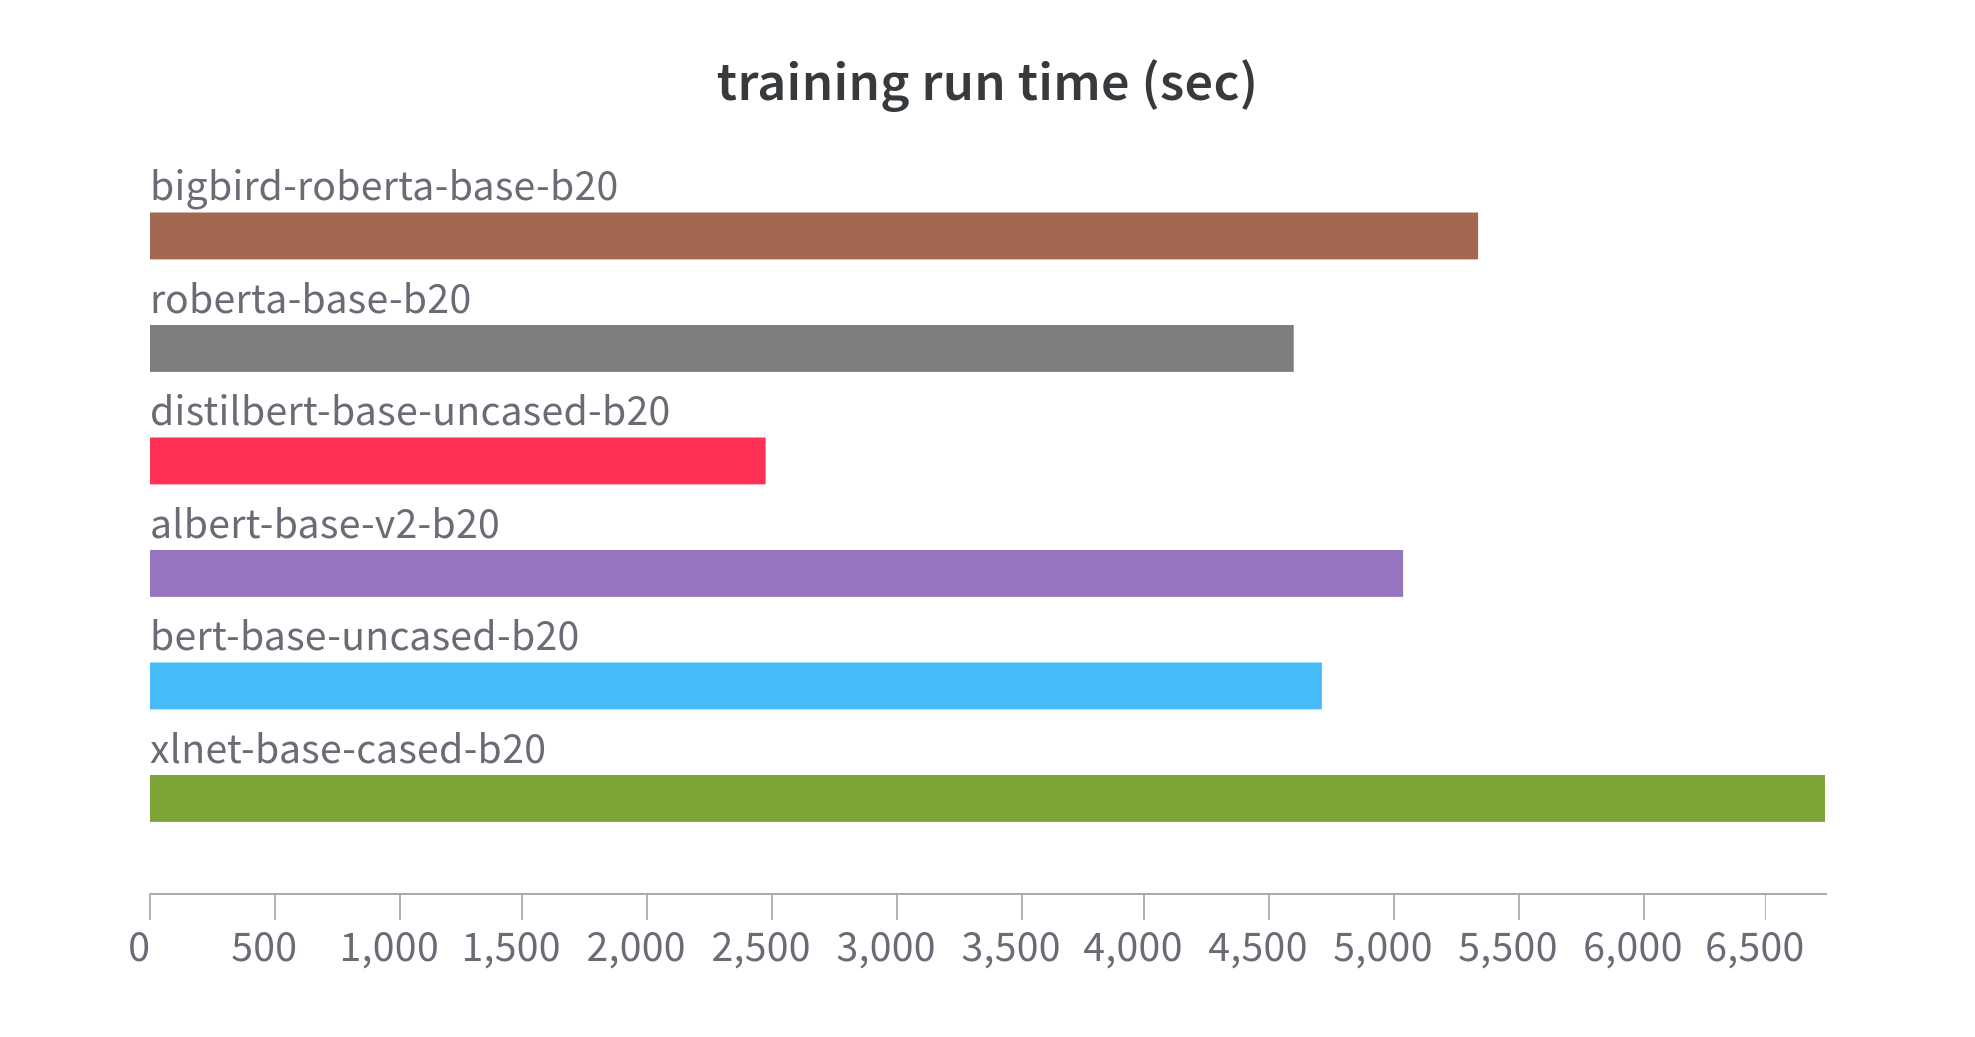
\includegraphics[scale=0.13]{train_time.png}
    \caption[Comparison]{Training time of each LM.}
    \label{fig:train_time}
\end{figure}

\section{Conclusion}

\section{Acknowledgements}
We would like to thank Massinissa Yebka for providing us with the computational power that made our calculations possible in a short time-frame.

\bibliographystyle{unsrt}
\bibliography{ref}


%\begin{figure}[htp]
%    \centering
%    \includegraphics[scale=0.37]{clustering_algo.png}
%    \caption{Prototype Clustering algorithm.}
%    \label{fig:clustering_algo}
%\end{figure}

\end{document}
